\section{How SSU-ALIGN's default alignment masks were determined}
\label{sec:masks}

This section describes how the default alignment masks used by
SSU-ALIGN were determined. There are three default masks,
one for each of the three default models: archaea, bacteria and
eukarya.

The masks were determined based on large datasets
of SSU sequences. Specifically, subsets of all the SSU sequences in
the  January 24, 2010 release of the GREENGENES database 
\cite{DeSantis06} and the \emph{Ref} set of SSU rRNA sequences from
release 100 of the SILVA database
\cite{Pruesse07} were used. Table~\ref{tbl:ggsil} includes statistics
on these alignments. 

The first step towards determining the masks was to run
\prog{ssu-align} with the \prog{--no-align} option on the combined
SILVA \emph{Ref} and GREENGENES unaligned
datasets, in FASTA format. If the combined dataset is in the file
\prog{ggsil.fa}, this could be reproduced using the command:

\user{ssu-align --no-align ggsil.fa ggsil}

From this, three new FASTA files are created in the new directory
\prog{ggsil/}: \prog{ggsil.archaea.fa}, \\ \prog{ggsil.bacteria.fa},
and \prog{ggsil.eukarya.fa}, 
the predicted set of archaeal, bacterial and eukaryotic
SSU sequences (possibly with some of the original
GREENGENES or SILVA sequence trimmed away from
the ends). 

Next, I used Robert Edgar's fast UCLUST tool (version 1.0.50) to
remove redundancy from each of these sets of sequences. Specifically, for
archaea, I executed the following three \prog{uclust} commands:

\user{uclust1.0.50\_linuxi86\_64 --sort ggsil.archaea.fa --output ggsil.sorted.archaea.fa}

\user{uclust1.0.50\_linuxi86\_64 --input ggsil.sorted.archaea.fa --uc \\  ggsil.f97.archaea.uc --id 0.97}

\user{uclust1.0.50\_linuxi86\_64 --input ggsil.sorted.archaea.fa --uc2fasta \\ ggsil.f97.archaea.uc --types S --output ggsil.f97.archaea.fa}

The final output file is \prog{ggsil.f97.archaea.fa}. This file has
been filtered to 97\% identity, i.e. each sequence should be at least
3\% different from all other sequences in this dataset. I repeated the
same procedure for the bacterial an eukaryotic datasets that were
output from the initial \prog{ssu-align} step as well.

I then created alignments of these datasets using
\prog{ssu-align}. For example, for the archaeal dataset, I executed: 

\user{ssu-align --no-search -n archaea ggsil.f97.archaea.fa arc4mask}

This generates the alignment \prog{arc4mask.archaea.stk} in the
directory \prog{arc4mask/}.  The final step was to execute
\prog{ssu-mask} on these alignments. By default, \prog{ssu-mask} will
examine the posterior probabilities in the alignment file to determine
a mask which defines which consensus columns to keep and which to
remove. Any consensus column for which 95\% of the sequences that do
not have a gap in the column have a posterior probability of at least
0.95 will be kept by \prog{ssu-mask}, all others will be removed. 

% original data from:
% /groups/eddy/home/nawrockie/notebook/10_0216_ssu_default_masks/00LOG
% on March 04.
%                               ********* 
%                                 F=0.97   F=0.95  F=0.90
%archaea                          
%ggsilR nseq:          23197        3853    2408     916
%ggsilR ncols kept:     1382        1376    1377    1364
%
%bacteria
%ggsilR nseq:         739075      118742   56554   17653
%ggsilR ncols kept:     1393        1376    1367    1343
%
%eukarya
%ggsilR nseq:          47442       12745    8194    3388
%ggsilR ncols kept:     1418        1343    1286    1141
%                               ********
%                                default
%                             SSU-aLIGN 0.1
%
%
%%%%%%%%%%%%%%%%%%%%%%%%%%%%%%%%%%%%%%%%%%%%%%%%%%%%%%%%
% Getting diagrams of the masks ON THE GGSILR ALIGNMENTS:
%
% Alignments and masks are in:
% /groups/eddy/home/nawrockie/notebook/10_0216_ssu_default_masks/masks/final_masks_strat5_ggsilR
% 
% Drawing dall figs logged in:
% /groups/eddy/home/nawrockie/notebook/10_0322_ssu_auto_merge/00LOG
% 
\begin{table}[hb]
\begin{center}
\begin{tabular}{r|rr|rr}
         & num seqs   & num seqs & \multicolumn{2}{c}{mask} \\ \cline{4-5}
domain   & unfiltered & filtered & included & excluded \\ \hline
archaea  & 23197      & 3853     & 1376     & 132 \\
bacteria & 739075     & 118742   & 1376     & 212 \\
eukarya  & 47442      & 12475    & 1343     & 538 \\ 
\end{tabular}
\caption{Statistics on the alignments used to determine the default
  SSU-ALIGN 0.1 alignment masks. The alignments were derived
  from the GREENGENES \cite{DeSantis06} and SILVA
  \cite{Pruesse07} databases as described in the text.}
\label{tbl:ggsil}
\end{center}
\end{table}

The default archaeal, bacterial and eukaryotic masks are shown in
figures~\ref{fig:mask-arc}, \ref{fig:mask-bac}, \ref{fig:mask-euk},
respectively. Each of theses figures includes two diagrams of the mask
displayed on the consensus secondary structure of the corresponding
model. The diagrams on the left of each figure show excluded positions
in pink, and included positions as black. The diagrams on the right
show excluded positions as open circles, and included positions as
solid squares, with positions colored by deletion (gap) frequency in
the filtered alignments used for determining the masks. Gray and dark
blue positions are never or rarely gaps; orange and red positions are
often gaps. Notice that nearly all of the positions that are excluded
by the mask are themselves or are nearby positions that are often
gaps. This is intuitive: alignment ambiguity increases (alignment
confidence decreases) in parts of SSU that tolerate insertions and
deletions because it becomes more difficult to determine which
exact nucleotides are homologous between different sequences in these
regions. Section~\ref{sec:background-pp},
page~\pageref{sec:background-pp} includes further discussion on
alignment ambiguity.

\begin{sidewaysfigure}
  \begin{center}
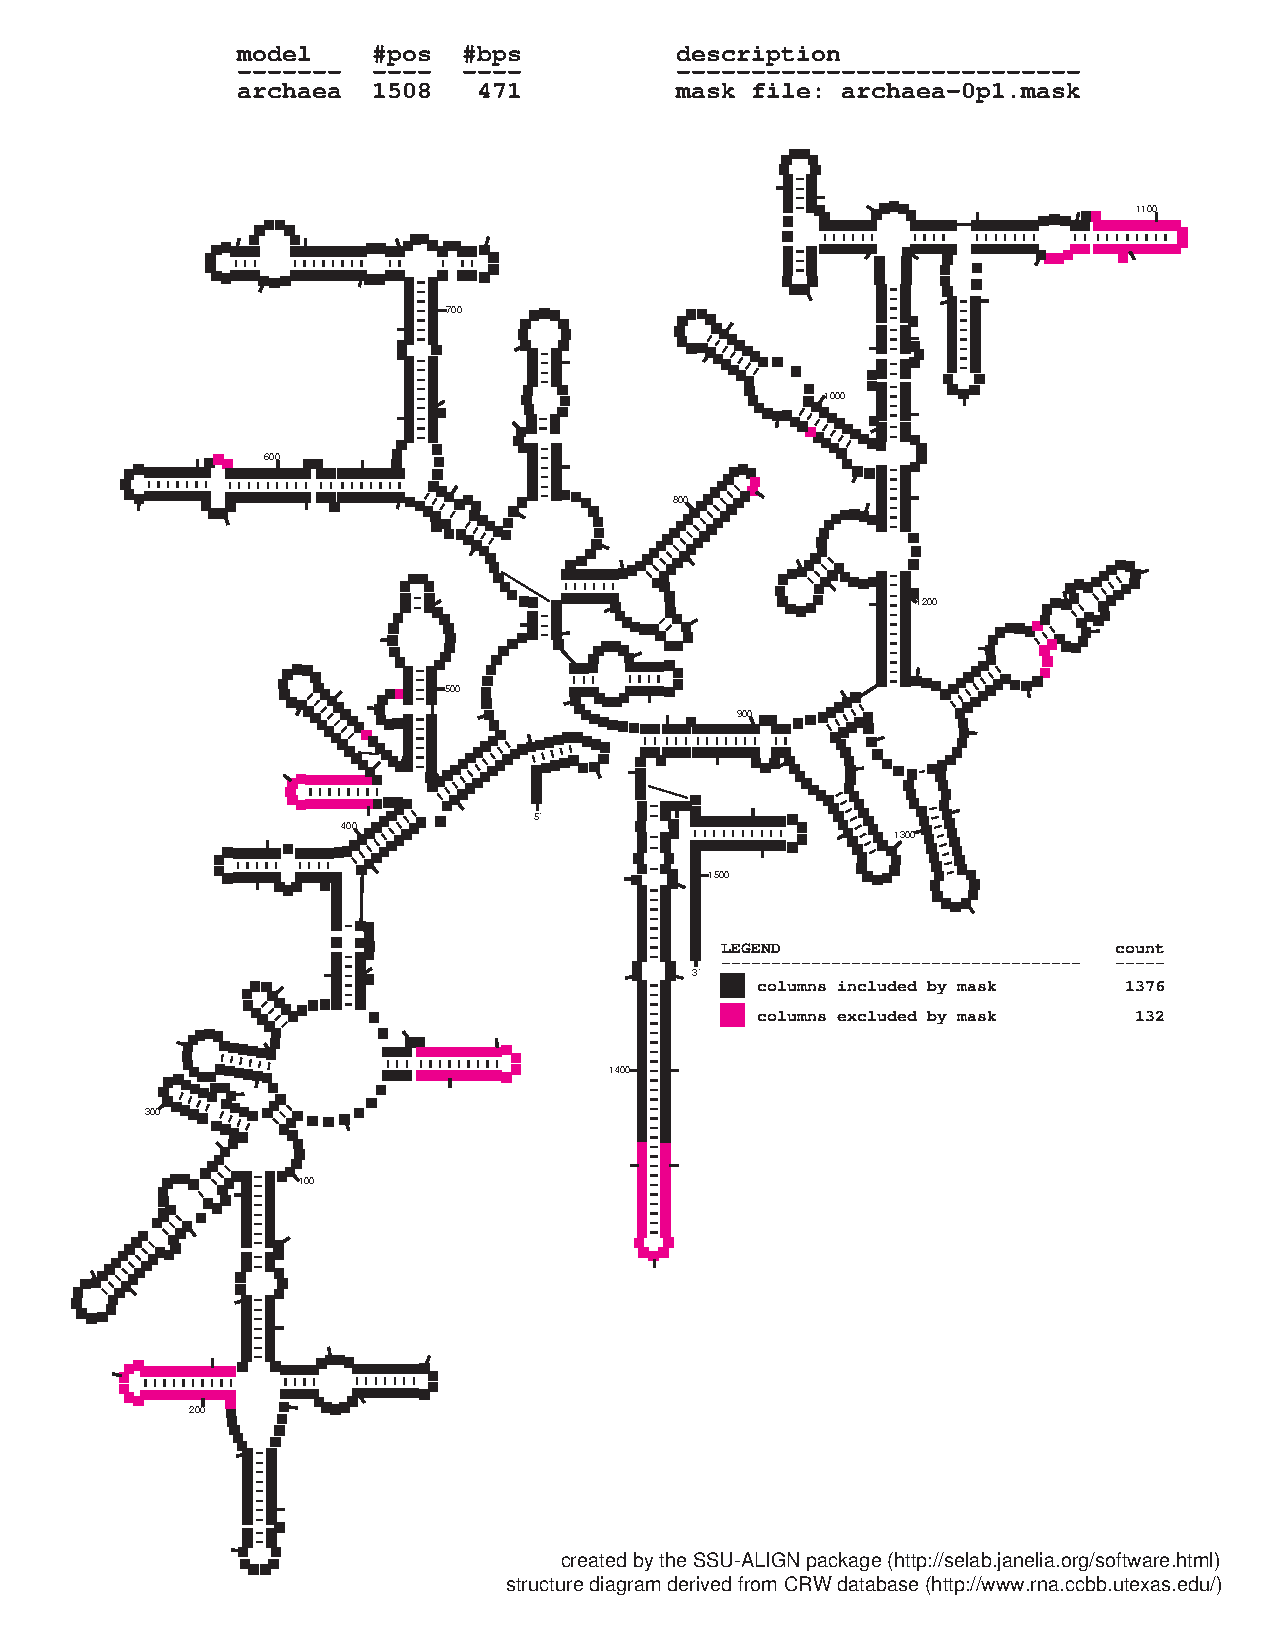
\includegraphics[width=4.2in]{Figures/archaea-0p1-mask}
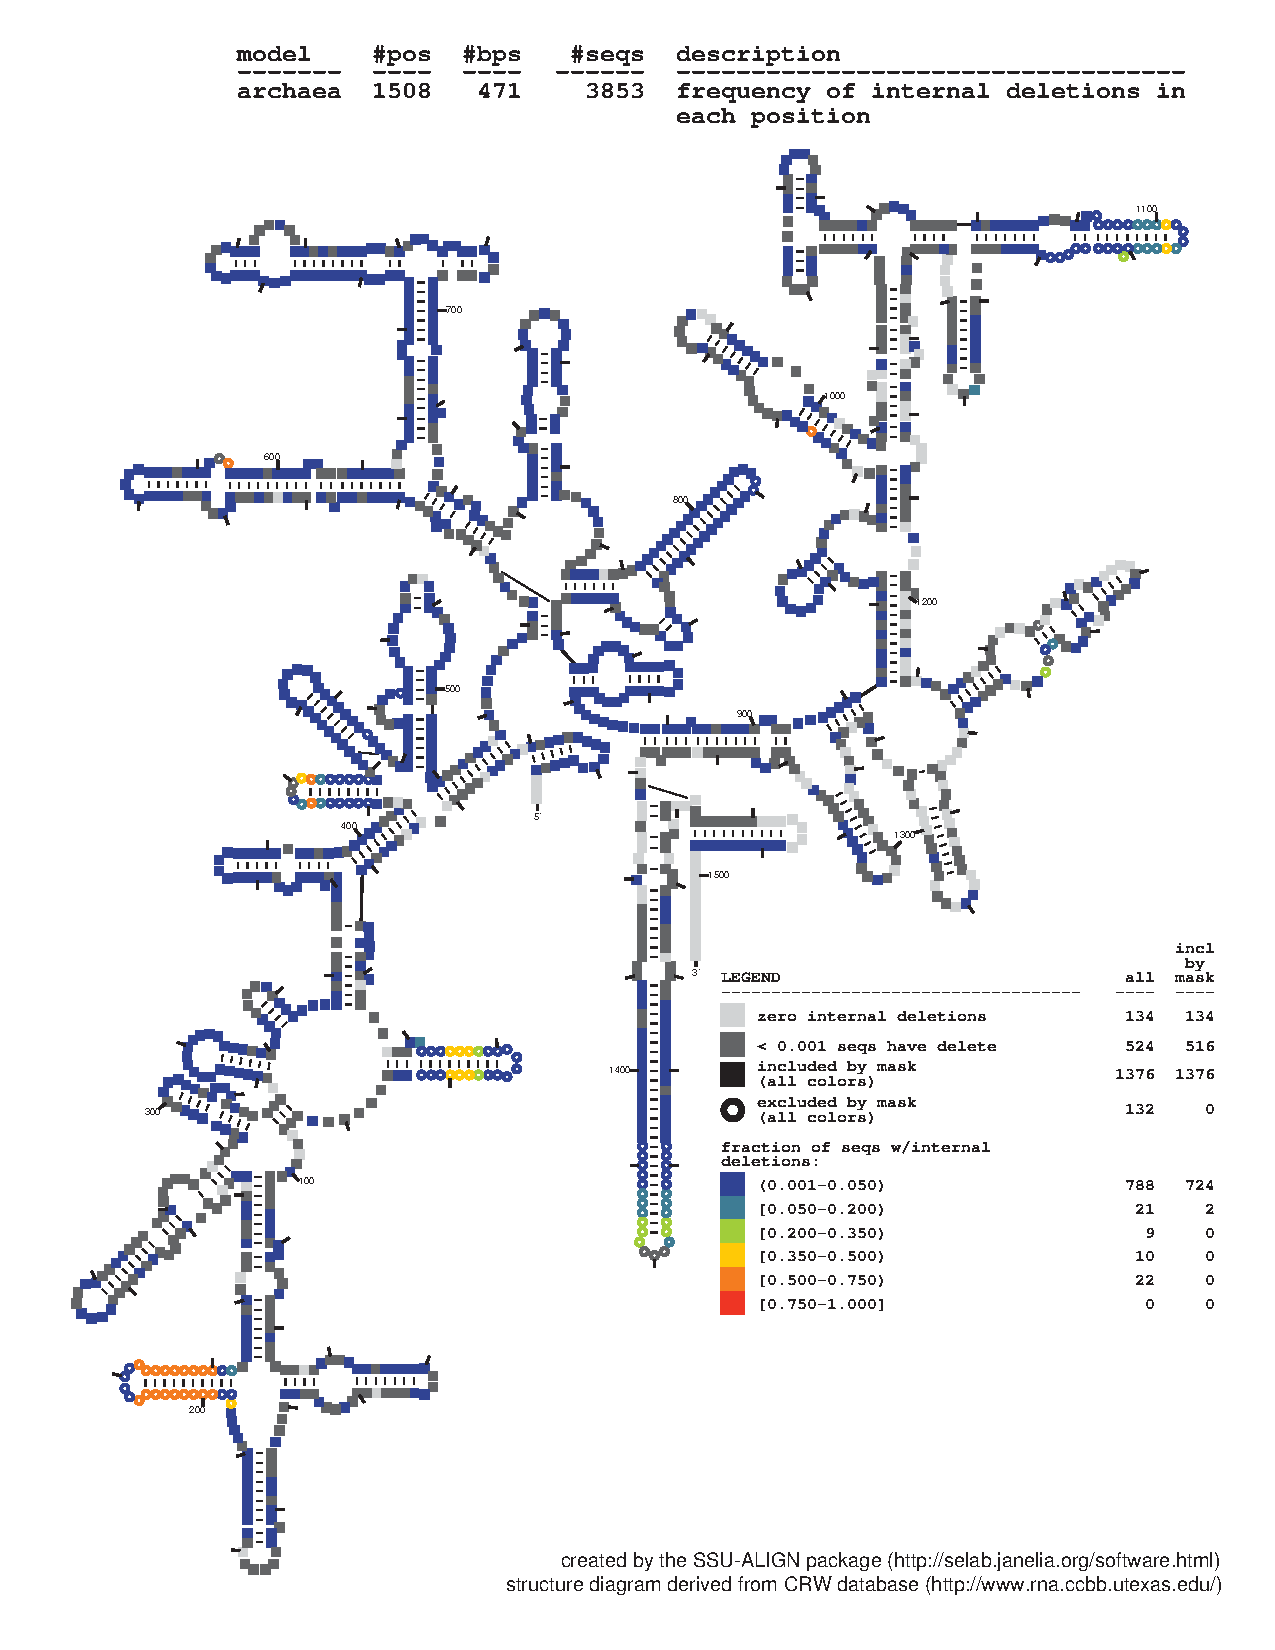
\includegraphics[width=4.2in]{Figures/archaea-ggsilR-dint-wmask}
  \end{center}
\caption{\textbf{Two diagrams of the default archaeal mask.} Left: pink positions are excluded,
  black positions are included. Right: Open circles are excluded,
  filled squares are included. Positions are colored based on
  frequency of deletions (gaps) in the filtered alignment of archaea
  from GREENGENES and SILVA \emph{Ref} (see text) as
  indicated in the legend.}
\label{fig:mask-arc}
\end{sidewaysfigure}

\begin{sidewaysfigure}
  \begin{center}
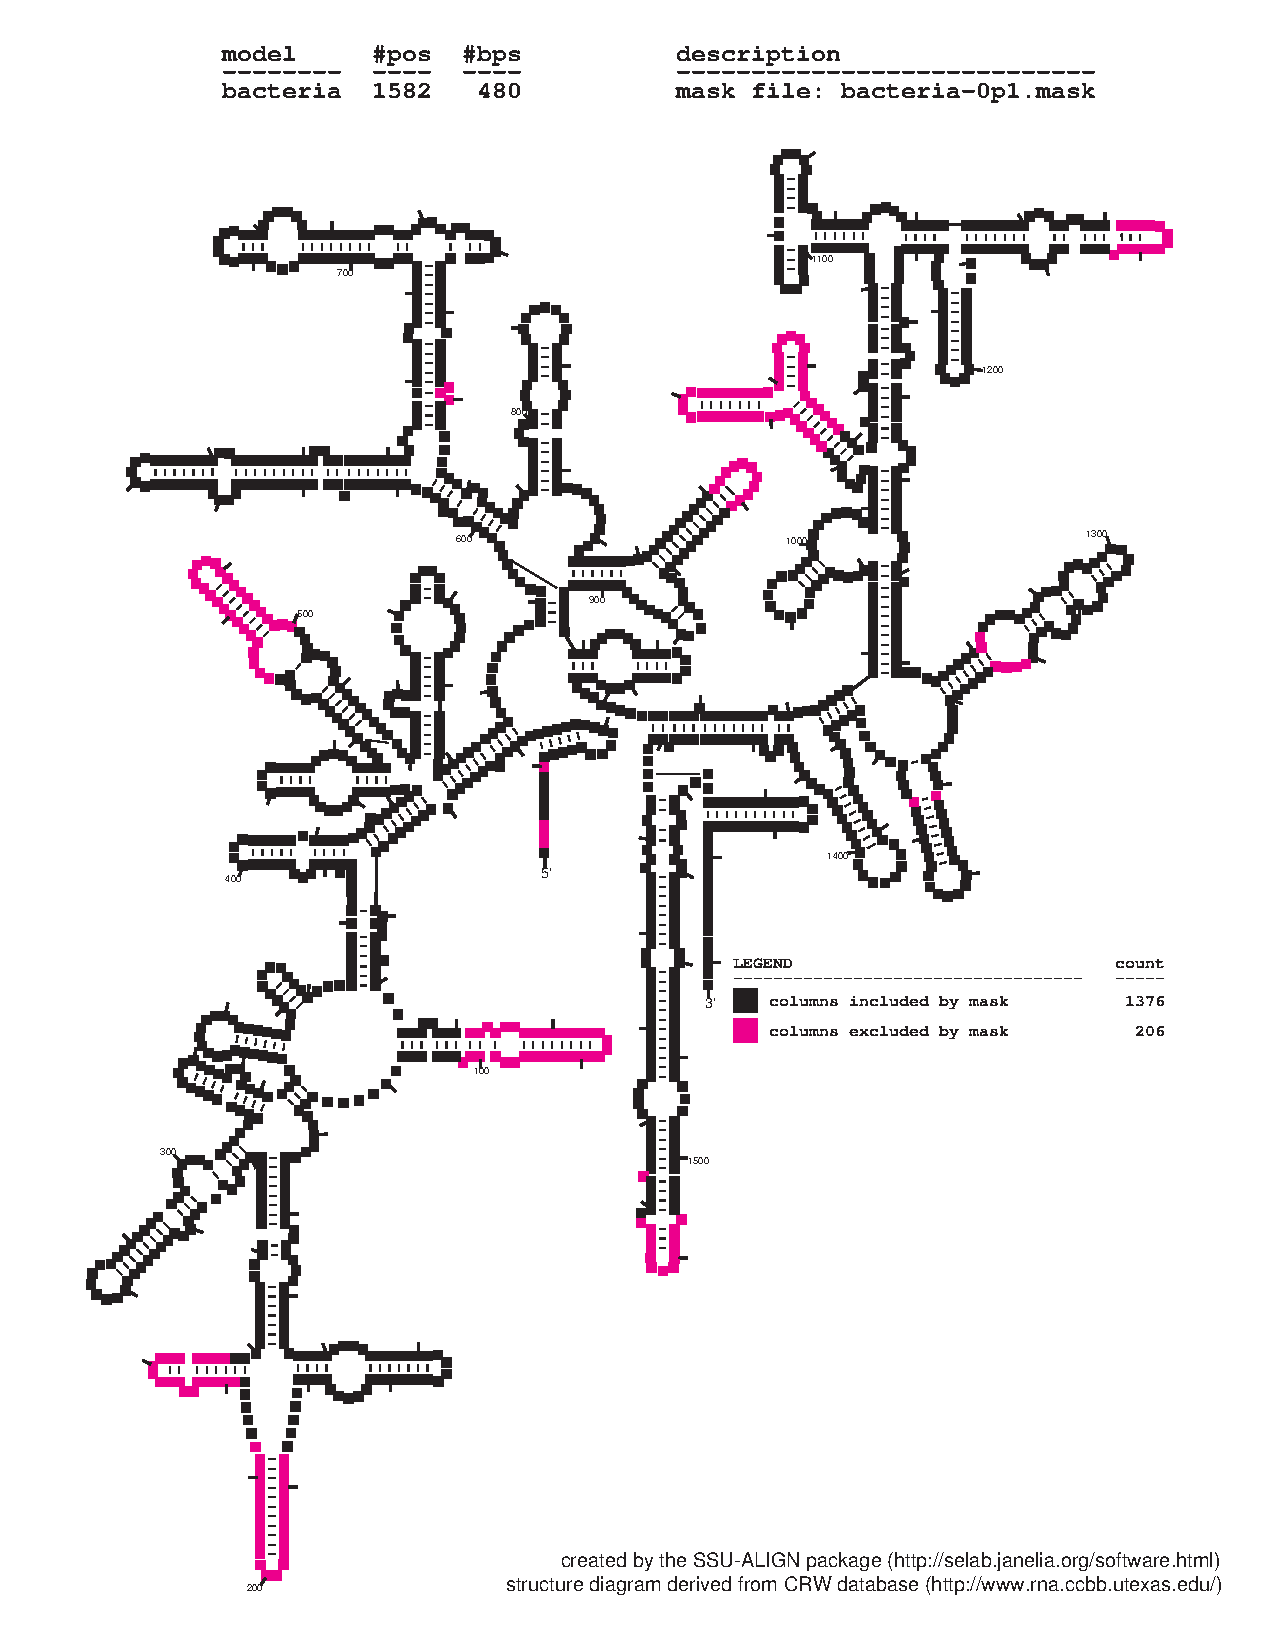
\includegraphics[width=4.2in]{Figures/bacteria-0p1-mask}
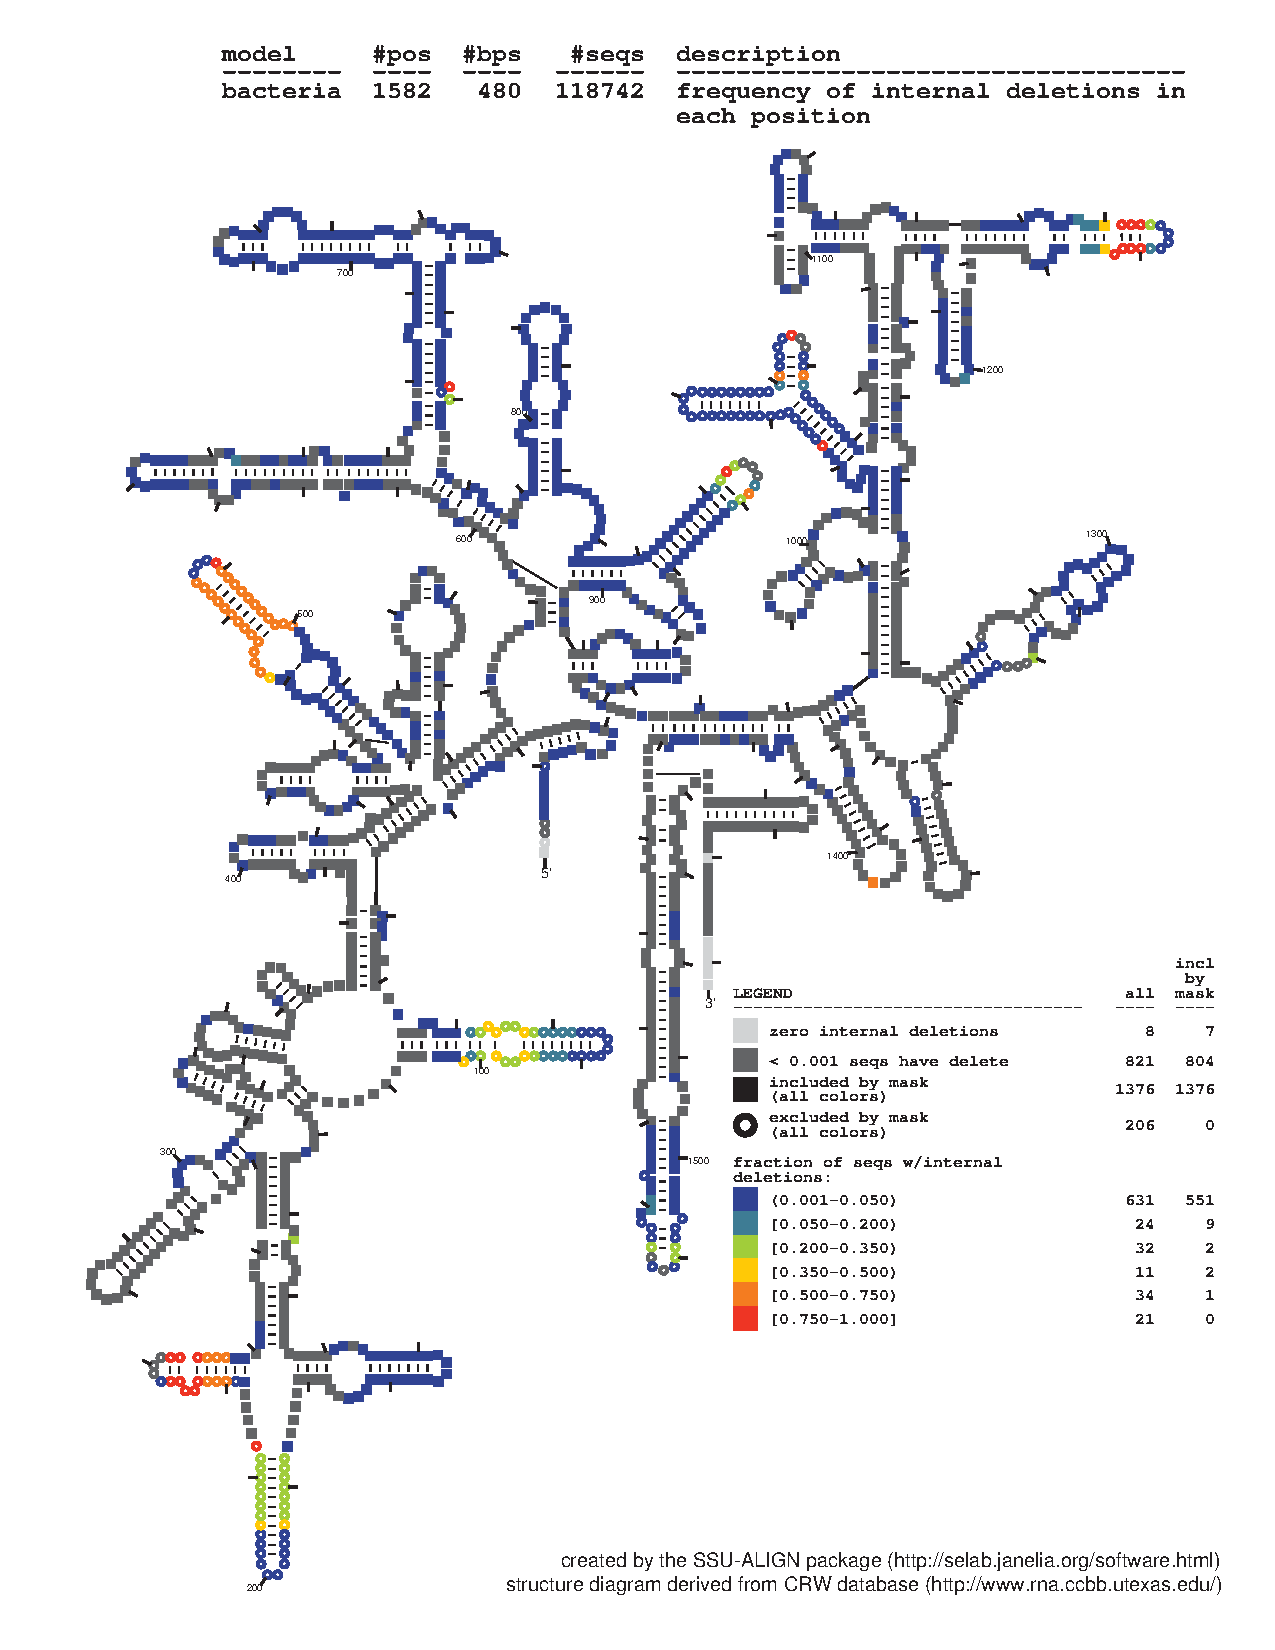
\includegraphics[width=4.2in]{Figures/bacteria-ggsilR-dint-wmask}
  \end{center}
\caption{\textbf{Two diagrams of the default bacterial mask.} Left: pink positions are excluded,
  black positions are included. Right: Open circles are excluded,
  filled squares are included. Positions are colored based on
  frequency of deletions (gaps) in the filtered alignment of bacteria
  from GREENGENES and SILVA \emph{Ref} (see text) as
  indicated in the legend.}
\label{fig:mask-bac}
\end{sidewaysfigure}

\begin{sidewaysfigure}
  \begin{center}
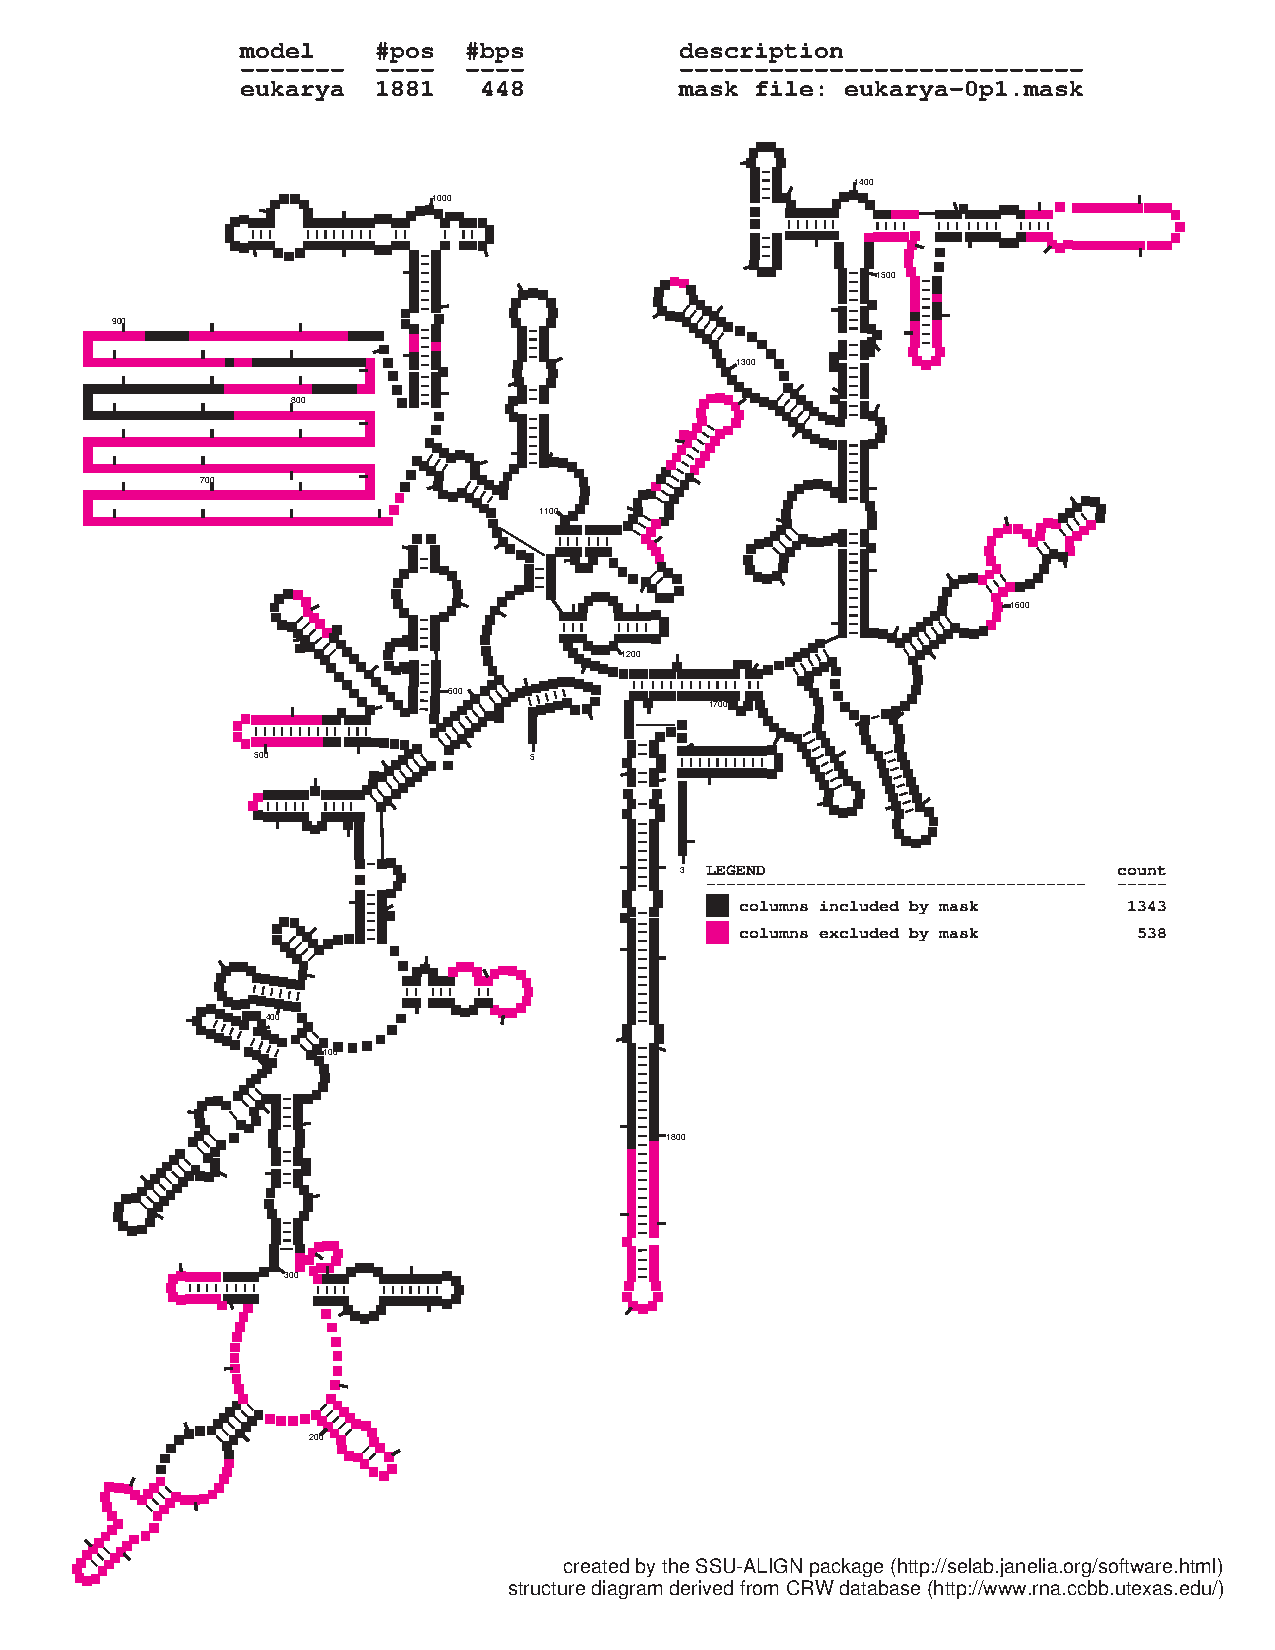
\includegraphics[width=4.2in]{Figures/eukarya-0p1-mask}
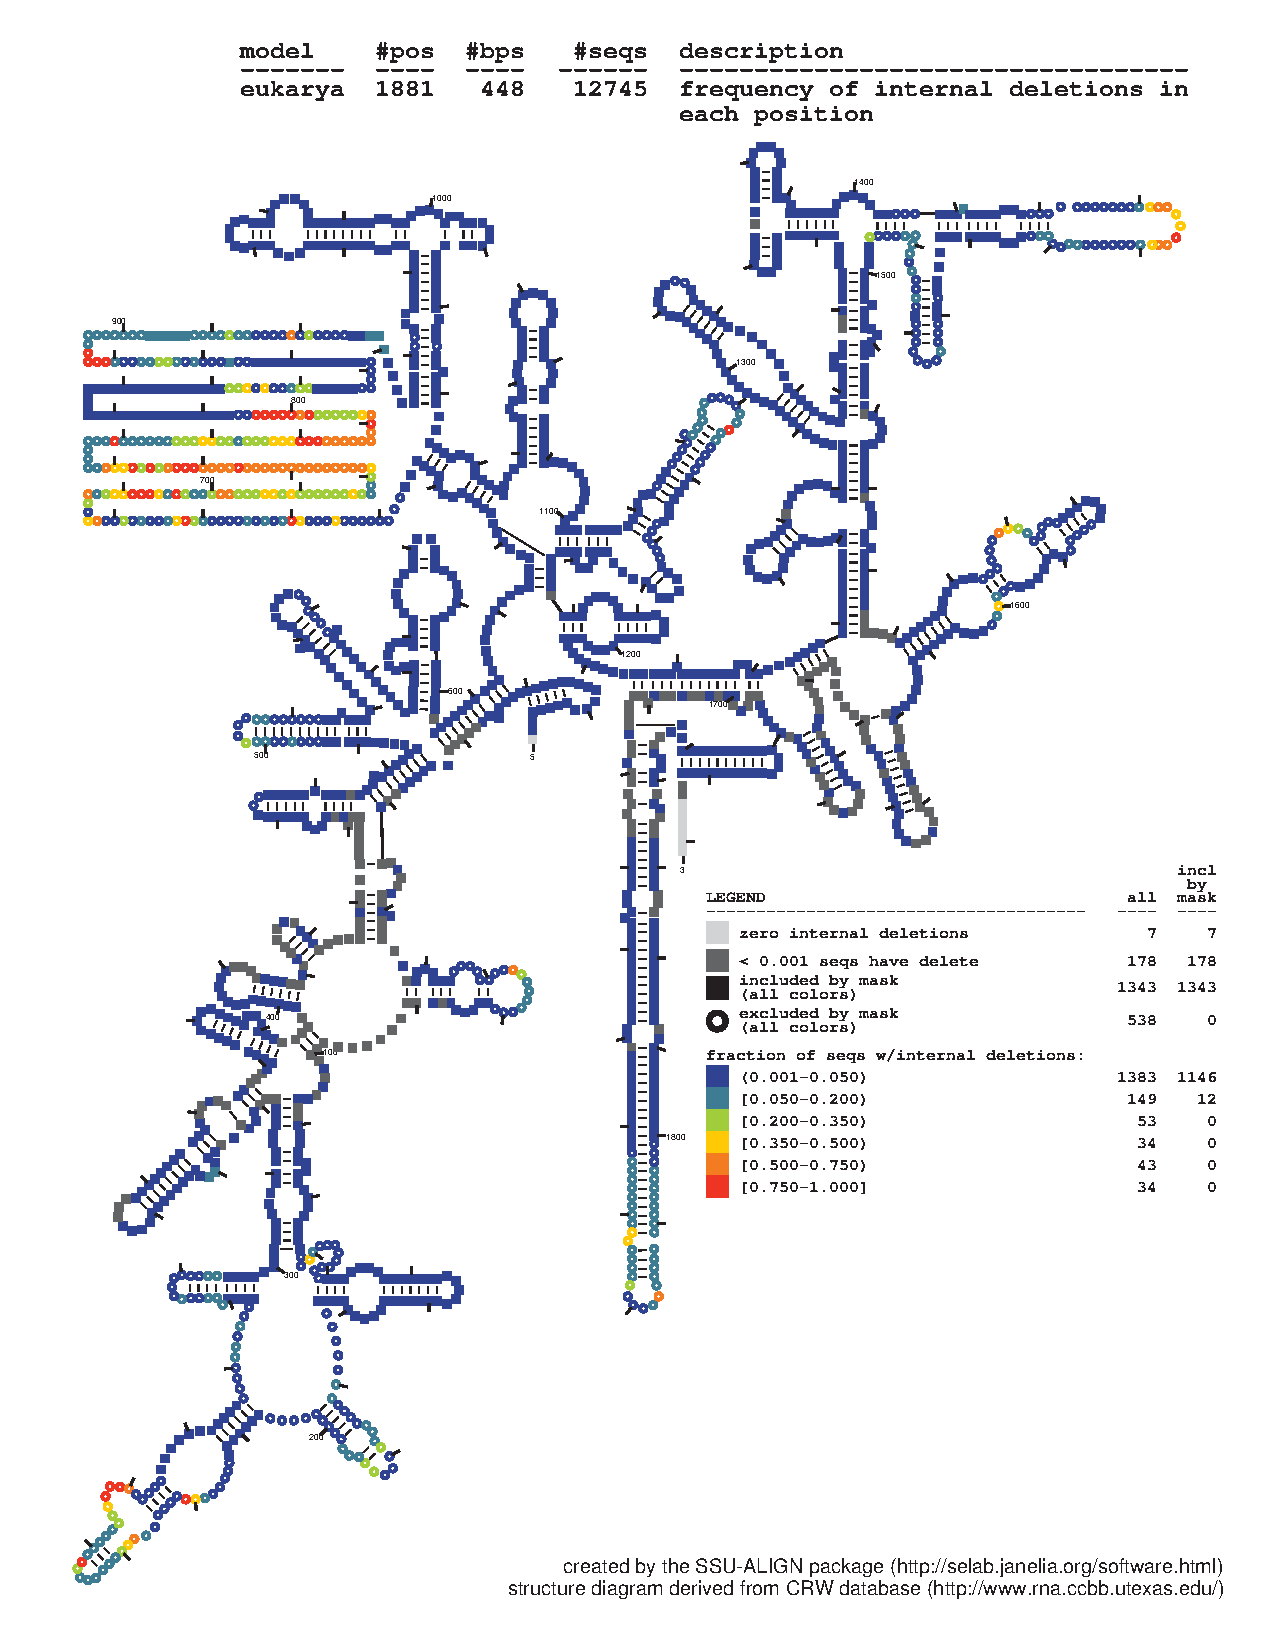
\includegraphics[width=4.2in]{Figures/eukarya-ggsilR-dint-wmask}
  \end{center}
\caption{\textbf{Two diagrams of the default eukaryotic mask.} Left: pink positions are excluded,
  black positions are included. Right: Open circles are excluded,
  filled squares are included. Positions are colored based on
  frequency of deletions (gaps) in the filtered alignment of eukarya
  from GREENGENES and SILVA \emph{Ref} (see text) as
  indicated in the legend.}
\label{fig:mask-euk}
\end{sidewaysfigure}
